\documentclass{article}

\usepackage{booktabs}
\usepackage{multirow}
\usepackage{amsmath}
\usepackage{hyperref}
\usepackage{overpic}
\usepackage{amssymb}

\usepackage[accepted]{dlaiml2026}

%%% STUDENTS: FILL IN WITH YOUR OWN INFORMATION
\dlaititlerunning{Not All Compression Is Equal: Rank Separates Memorisation from Generalisation in Grokking}

\begin{document}

\twocolumn[
%%% STUDENTS: FILL IN WITH YOUR OWN INFORMATION
\dlaititle{Not All Compression Is Equal: Rank Separates Memorisation from Generalisation in Grokking}

\begin{center}\today\end{center}

\begin{dlaiauthorlist}
%%% STUDENTS: FILL IN WITH YOUR OWN INFORMATION
\dlaiauthor{Giovanni Ciarravano}{}
\end{dlaiauthorlist}

%%% STUDENTS: FILL IN WITH YOUR OWN INFORMATION
\dlaicorrespondingauthor{Giovanni Ciarravano}{ciarravano.1989209@studenti.uniroma1.it}

\vskip 0.3in
]

\printAffiliationsAndNotice{}

\begin{abstract}
	During grokking a network memorises its training data long before it generalises. In
	between, training accuracy is saturated and cannot tell the two phases apart; we ask
	whether post-training compression can. Applying SVD rank truncation, magnitude pruning and uniform quantisation at matched
	points on the trajectory, rank provides the strongest separation (gap $+0.86$, against $+0.38$
	and $+0.22$). A threshold on the minimal viable rank, calibrated on one condition, transfers unchanged
	to another ($4/4$) with no false positive on four controls, and holds for every threshold
	in $[11,31]$. We find no significant evidence that it arrives before the accuracy jump
	(median $-130$ steps, sign test $p = 0.15$, $n = 12$). Code:
	\url{https://github.com/GiovanniCiarra/DLAI-Project2026}.
\end{abstract}

\section{Introduction}

Grokking \cite{power2022} is a phenomenon in which a network reaches perfect
training accuracy long before it generalises. In between --- thousands of optimisation
steps --- the training signal is saturated and says nothing about whether the network
found an algorithm or a lookup table; telling them apart normally requires a held-out
set. We ask whether compression can instead: a lookup table needs every entry stored
precisely, whereas a rule tolerates perturbation. If so, compressing the weights and
re-running the \emph{training} data suffices, with no held-out data and no knowledge of
the expected circuit.
Our contributions are three, one negative. \textbf{(i)} Of three compression operators applied at matched positions, rank truncation
separates the two phases more sharply than pruning or quantisation. \textbf{(ii)} A threshold on the minimal viable rank $r^\star$, calibrated on one
condition, transfers unchanged to another and produces no false positive on the
controls, over a wide interval of thresholds. \textbf{(iii)} Several accounts describe grokking as coinciding with a drop in model
complexity \cite{liu2023,varma2023}, which invites the question of an
early warning. For the rank axis, we find no significant evidence of one.

\section{Related work}

Grokking on modular arithmetic was introduced by \citet{power2022}, and
\citet{nanda2023progress} showed that its generalising solution is a Fourier circuit, and proposed progress measures that require knowing which
frequencies it uses.
Subsequent work linked grokking to reductions in complexity --- including linear
mapping number, weight norm, circuit efficiency, and sparse subnetworks
\cite{liu2023,liu2023omnigrok,varma2023,merrill2023} ---
while \citet{minegishi2025bridging} studied lottery-ticket-style pruning and
retraining. \citet{junior2025grokking} showed that regularising towards sparse or
low-rank weights can itself induce grokking. Other approaches use input robustness
or perturbation-based signals \cite{tan2024,schiff2021},
while \citet{li2026} monitor generalisation from training data alone in
mixture-of-experts language models.
Our work is operational and post-training: we compare rank truncation, magnitude
pruning and quantisation without retraining, and test whether the resulting
functional robustness can distinguish memorisation from generalisation using only
training data at detection time.

\section{Method}

\textbf{Setup.} A one-layer transformer ($d_{\text{model}}{=}128$, $4$ heads,
$d_{\text{mlp}}{=}512$, no LayerNorm, dropout or biases; $222$k parameters) on
$(a{+}b) \bmod 97$, full-batch AdamW ($\text{lr}{=}10^{-3}$, $\beta{=}(0.9,0.98)$, weight decay $1.0$ except
in \textsc{nc\_wd0}), $30{,}000$ steps ($40{,}000$ for \textsc{long}). A scan over the training fraction recovers three of the four regimes of
\citet{liu2022towards} and fixes the conditions of Table~\ref{tab:main}; the scan itself is in the
appendix (Table~\ref{tab:phases}).
The controls are complementary: \textsc{nc\_wd0} rules out long training as the cause,
while \textsc{nc\_mem} shares the weight decay of \textsc{main}, so a by-product of
weight shrinkage would appear there too. Per-tensor absmax quantisation is moreover
scale-invariant, so smaller weights do not quantise more easily.

\textbf{Operators and measure.} Applied post hoc to the weight matrices with no
retraining: uniform symmetric per-tensor quantisation at $b$ bits; one-shot global
magnitude pruning at sparsity $s$; per-matrix SVD truncation to rank $r$, the optimal
rank-$r$ approximation in Frobenius norm (Eckart--Young). We record retained \emph{training} accuracy: test accuracy never enters the computation
of $r^\star$ or of the detector once calibrated, and is used only to label the
generalisation phase. We define
\[
r^\star(\theta) = \min \{\, r : \mathrm{acc}_{\text{train}}(\mathrm{trunc}_r(\theta))
\geq 0.9 \cdot \mathrm{acc}_{\text{train}}(\theta) \,\},
\]
for checkpoints that have memorised ($\mathrm{acc}_{\text{train}} \geq 0.99$), since
before that there is no learned function to preserve. The $0.9$ threshold was fixed a
priori; we evaluate $r^\star$ at $2{,}564$ of $3{,}196$ checkpoints across $16$ runs.

\textbf{Anchors.} Per run we take the last checkpoint that has memorised but not
generalised ($\mathrm{acc}_{\text{test}} \leq 0.15$) and the final one --- they coincide
in the controls --- giving $12$ generalising and $16$ non-generalising anchors. The
first plateau checkpoint is excluded, lying near initialisation where any network is
high-rank.

\section{Results}

\textbf{Rank provides the strongest separation (Table~\ref{tab:main}, top).} At rank $16$ every
generalising anchor retains its full training accuracy, with zero variance across runs,
while the memorising ones drop to $0.14$. Test accuracy tracks it throughout the
sweep (appendix), so truncation degrades the computed function rather than selectively
removing generalisation: at rank $16$ the model retains $20\%$ of the parameters ($44$k of $222$k) in factored form at no measurable cost. The best gaps for pruning and quantisation
are two to four times smaller, with overlapping error bands. Quantisation in fact tracks weight decay: \textsc{nc\_wd0} is the most fragile of all
under it, since large outliers survive and inflate the per-tensor scale --- visible only
because of that control.

\begin{table}[h]
	\caption{\textbf{Top:} retained training accuracy at the operating points below,
		over $12$ generalising and $16$ memorising anchors (mean $\pm$ s.d.\ across runs). For rank we report $16$ rather than the maximum-separation level $14$
		($+0.88$), since at $16$ the generalising group has zero variance.
		\textbf{Bottom:} minimal viable rank and detection at $R_{\text{crit}}{=}25$, calibrated
		on \textsc{main} alone. \textsc{main}/\textsc{long}/\textsc{nc\_mem}/\textsc{nc\_wd0} use $30/25/20/30\%$ of the data, weight decay $1.0$ except \textsc{nc\_wd0}.}
	\label{tab:main}
	\vskip 0.00in
	\begin{center}
		\begin{small}
			\setlength{\tabcolsep}{4.5pt}
			\begin{tabular}{lccc}
				\toprule
				operator & gen. & mem. & gap \\
				\midrule
				rank $r{=}16$    & $\mathbf{1.000 \pm .000}$ & $0.137 \pm .115$ & $\mathbf{+0.86}$ \\
				prune $s{=}0.40$ & $0.783 \pm .185$ & $0.402 \pm .260$ & $+0.38$ \\
				quant.\ $3$ bit  & $0.450 \pm .186$ & $0.229 \pm .130$ & $+0.22$ \\
				\midrule
				condition & final $r^\star$ & min $r^\star$ & det. \\
				\midrule
				\textsc{main}    & $10$--$15$ & $9$--$11$  & $8/8$ \\
				\textsc{long}    & $10$--$14$ & $9$--$10$  & $4/4$ \\
				\textsc{nc\_mem} & $33$--$34$ & $32$       & $0/2$ \\
				\textsc{nc\_wd0} & $77$--$83$ & $61$--$62$ & $0/2$ \\
				\bottomrule
			\end{tabular}
		\end{small}
	\end{center}
	\vskip -0.30in
\end{table}


\textbf{Three populations (Table~\ref{tab:main}, bottom).} Along the trajectory $r^\star$ shows two distinct descents. The first, from
${\approx}70$ to ${\approx}35$, is consistent with weight decay driving it:
\textsc{nc\_mem} makes it without ever generalising, \textsc{nc\_wd0} does not. Below
${\approx}32$ the descent happens only under generalisation, and the controls' minima
over the trajectory are $32$ and $61$, so neither enters the generalising
band.
We detect with an absolute threshold, $t_{\text{detect}} = \min\{t : r^\star(t) \leq
R_{\text{crit}}\}$; a relative criterion would fail, since \textsc{nc\_mem} halves its
$r^\star$ without generalising. $R_{\text{crit}}$ is fixed in advance as the midpoint
between the largest final $r^\star$ ($15$) and the smallest plateau $r^\star$ ($35$)
over \textsc{main} alone. Every threshold in
$[11,31]$ separates perfectly; the break at $32$ is exactly the trajectory minimum of
\textsc{nc\_mem}. Calibration needs the labels of \textsc{main}; the detector does not.
\textsc{long} is a different condition (grokking at $13$--$26$k steps instead of
$4$--$9$k), so transferring the threshold unchanged is out-of-condition validation.

\textbf{But it does not fire early.} With $t_{\text{grok}}$ the first step at test
accuracy $\geq 0.5$, the median lead time is $-130$ steps and $9$ of $12$ runs are
negative, but an exact two-sided sign test on the paired design gives $p=0.15$. We do not reject the null. Magnitudes agree: in \textsc{main} the offsets span $-298$
to $+365$ steps against plateaus of $3{,}675$--$8{,}525$, below $10\%$. The detector can replace held-out labels after calibration, but we find no significant evidence that it anticipates grokking.

\textbf{Consistency with the Fourier circuit.} A spectral analysis of the digit embeddings
(appendix) gives $r^\star \geq 2k$ in $12/12$ runs, $k$ being the number of key
frequencies: two independent measures agree. No frequency is shared by all
runs, consistent with $r^\star$ reflecting the dimensionality of the computed circuit
rather than one solution --- and unlike spectral concentration it needs no prior
knowledge that the solution is Fourier.

\section{Discussion and limitations}

The choice of compression operator appears more discriminative than the amount: rank
truncation separates far better than pruning or quantisation. After calibration the
rank probe needs only training data, but its scope is one task, one prime, one
architecture, with a solution known to have low-dimensional structure. Whether $r^\star$ transfers to other tasks or model families is unknown, and
$R_{\text{crit}}$ depends on model width. The two-descent reading rests on
complementary controls rather than a continuum of weight-decay values. Finally,
lead-time inference is limited by the ${\approx}152$-step checkpoint spacing and
$n=12$: the null is not proof that no predictive signal exists.


\section*{Statement on the use of AI}\label{sec:ai}
%
Anthropic’s Claude was used as an assistant throughout the development of this project. It was used for literature exploration, discussion and refinement of the experimental design, implementation of the model and analysis code, debugging, figure generation, and writing and editing the report.

The project was developed through an iterative exchange with the AI. Claude helped me explore and understand the relevant literature, particularly the papers discussed in the Related Work section, and to assess how the ideas and results of this project relate to previous work. It also helped me evaluate and compare different project ideas before the final topic was selected, and supported me in understanding the underlying concepts and methodology of the chosen project. During development it proposed and refined several experimental ideas, including the phase-diagram scan, the complementary control conditions, the definition of $r^\star$, and the calibration protocol. I selected the final project direction, made the final methodological decisions, ran all experiments on my own hardware, inspected the outputs, and decided which results and analyses were retained in the final report.

Claude also assisted with the writing of the report. In particular, it helped improve the formality and correctness of the English, reformulate parts of the text, and reduce and reorganise the material so that the complete report could fit within the required two-page limit without removing essential content. The final selection of results, interpretation of the findings, claims, limitations, and overall presentation were my responsibility.


\bibliography{references.bib}
\bibliographystyle{dlaiml2026}

\section*{Appendix}

\begin{table}[H]
	\centering
	\caption{Phase diagram of the setup: seed $0$, $30{,}000$ steps, weight decay $1.0$.
		$t_{\text{mem}}$ is the first step with training accuracy $\geq 0.99$,
		$t_{\text{grok}}$ the first with test accuracy $\geq 0.5$. The main condition
		($30\%$) is the widest plateau that is not adjacent to the memorisation boundary.}
	\label{tab:phases}
	\vskip 0.0in
	\begin{small}
		\begin{tabular}{lrrrl}
			\toprule
			frac & examples & $t_{\text{mem}}$ & $t_{\text{grok}}$ & regime \\
			\midrule
			$0.20$ & $1881$ & $125$ & never & memorisation \\
			$0.25$ & $2352$ & $125$ & $17825$ & grokking \\
			$0.30$ & $2822$ & $125$ & $6775$ & grokking \\
			$0.35$ & $3293$ & $150$ & $3875$ & grokking \\
			$0.40$ & $3763$ & $150$ & $1175$ & comprehension \\
			\bottomrule
		\end{tabular}
	\end{small}
\end{table}

\textbf{Computation of $r^\star$.} By binary search over $r \in [1,128]$ (rank $128$ is
the identity for every tensor, so $r^\star$ is always defined). The search is exact only
if retention is monotone in $r$; this was verified on the full grid $1$--$128$ over a
sample of checkpoints spanning all conditions and training phases, with zero violations.
Checkpoints follow a hybrid grid: $120$ log-spaced points over the run plus $80$--$146$
linearly spaced across the transition window, chosen so that the spacing there is
$\approx152$ steps in every condition. Spectral concentration is $0.952 \pm 0.013$ for generalising runs
against $0.238 \pm 0.073$ for controls (white-noise level $6/48$); the mean margin
$r^\star - 2k$ is $+3.42$, and $27$ distinct key frequencies appear across the $12$ runs
with none shared by all.

\begin{figure}[H]
	\centering
	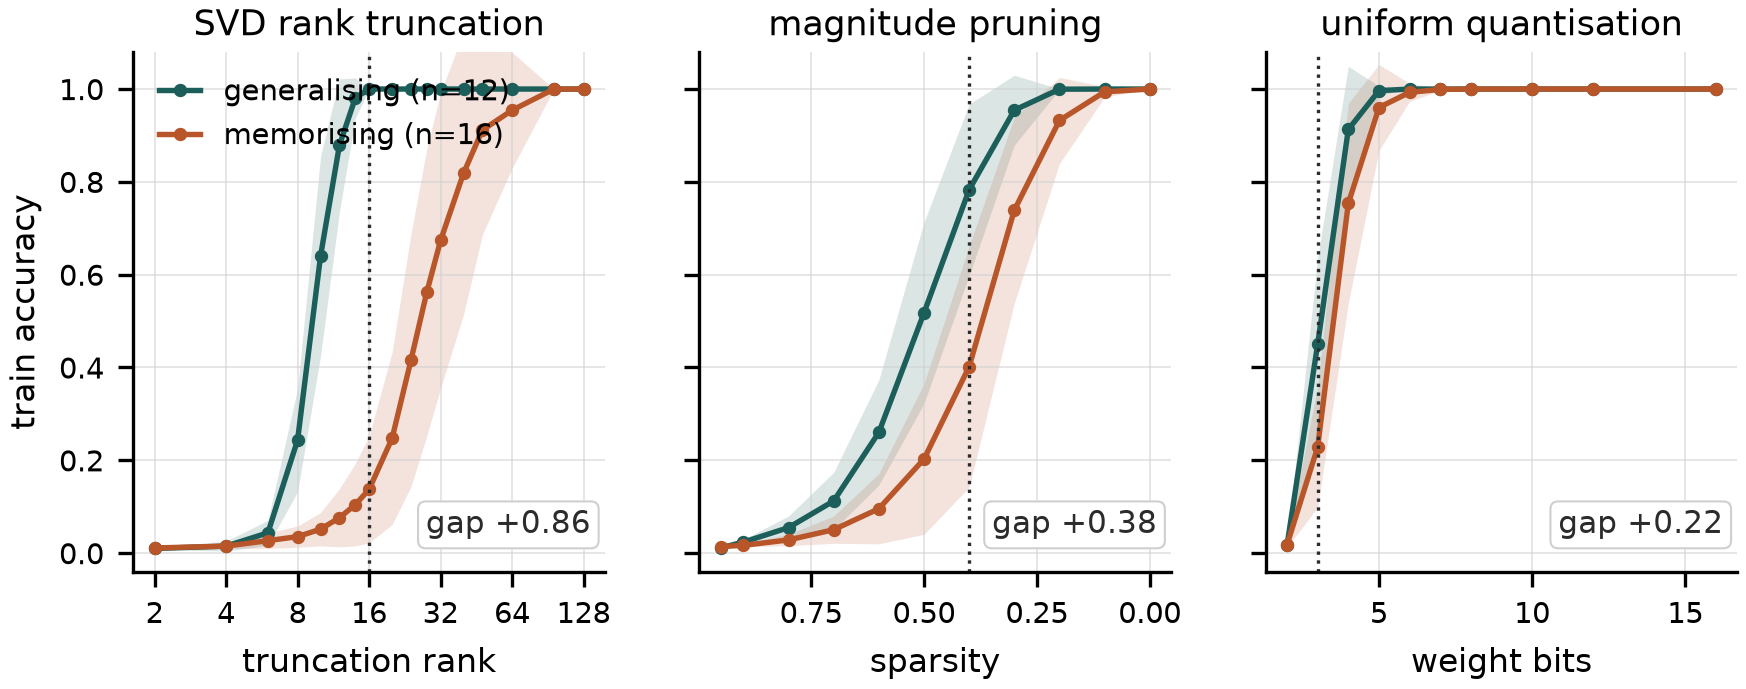
\includegraphics[width=\columnwidth]{../figures/fig1_operators.png}
	\caption{Retained training accuracy under the three operators, over $12$ generalising
		and $16$ memorising anchors; bands are one standard deviation across runs. Compression
		is strongest on the left in all panels; dotted lines mark the reported operating points. The gap is $+0.86$ for rank, $+0.38$ for pruning, $+0.22$ for quantisation.}
\end{figure}

\begin{figure}[H]
	\centering
	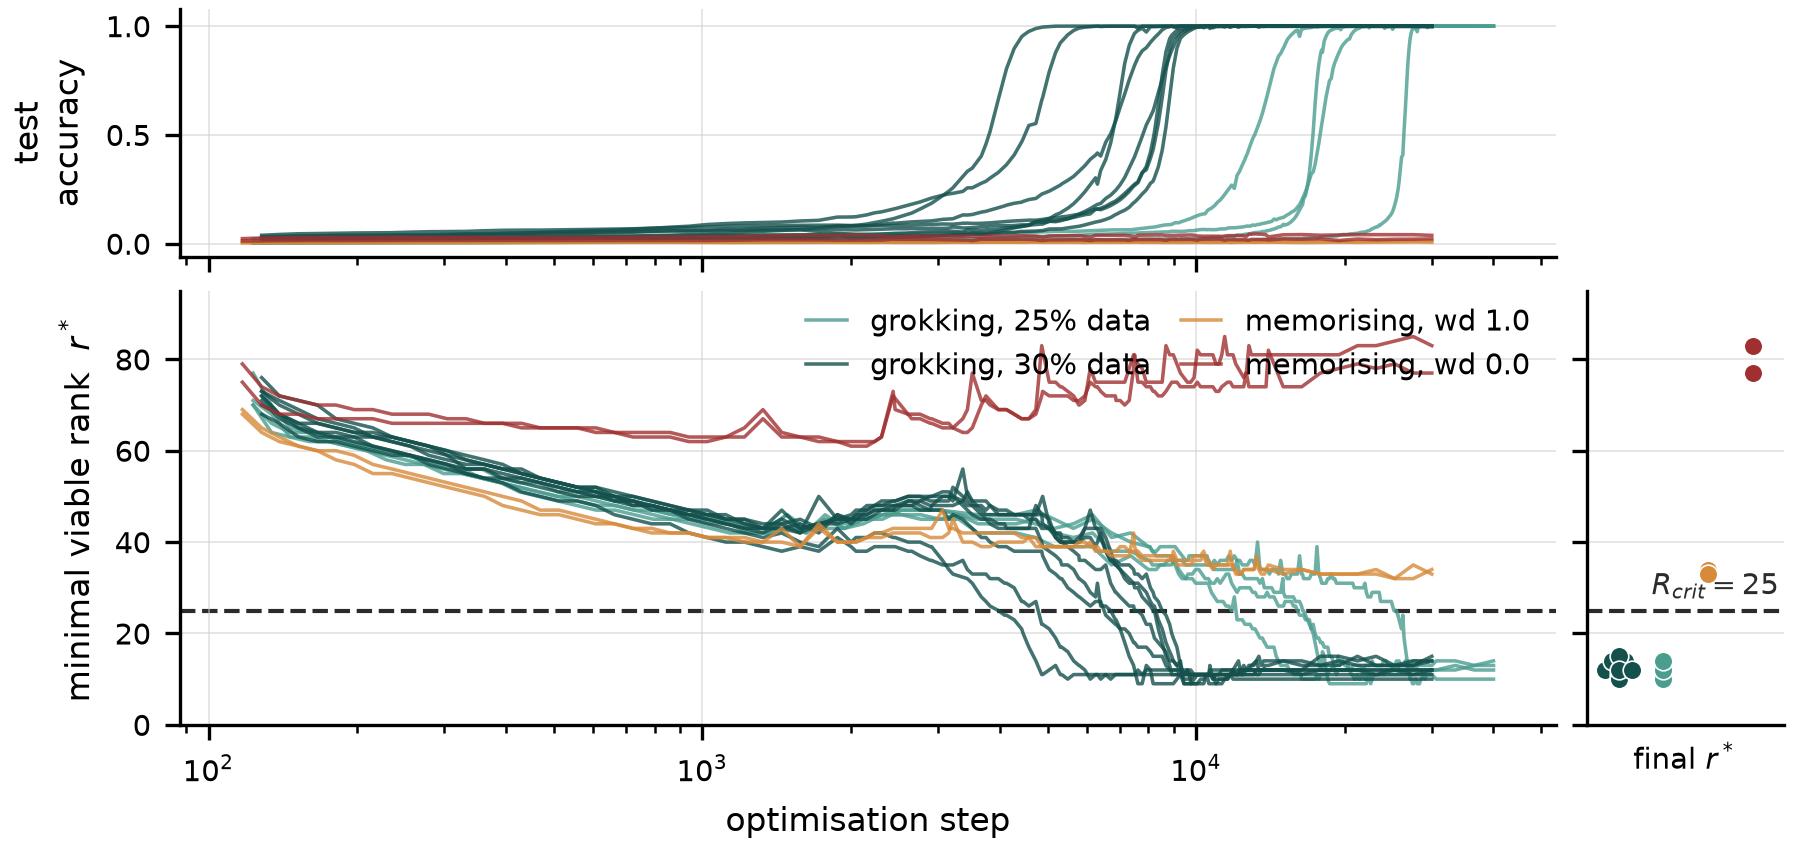
\includegraphics[width=\columnwidth]{../figures/fig2_trajectories.png}
	\caption{Test accuracy (top) and minimal viable rank (bottom) along training, all $16$
		runs; the side strip repeats the final $r^\star$. Without weight decay $r^\star$ stays
		above $60$; with weight decay but without generalisation it stops near $33$; only
		generalising runs cross $R_{\text{crit}}$.}
\end{figure}

\begin{figure}[H]
	\centering
	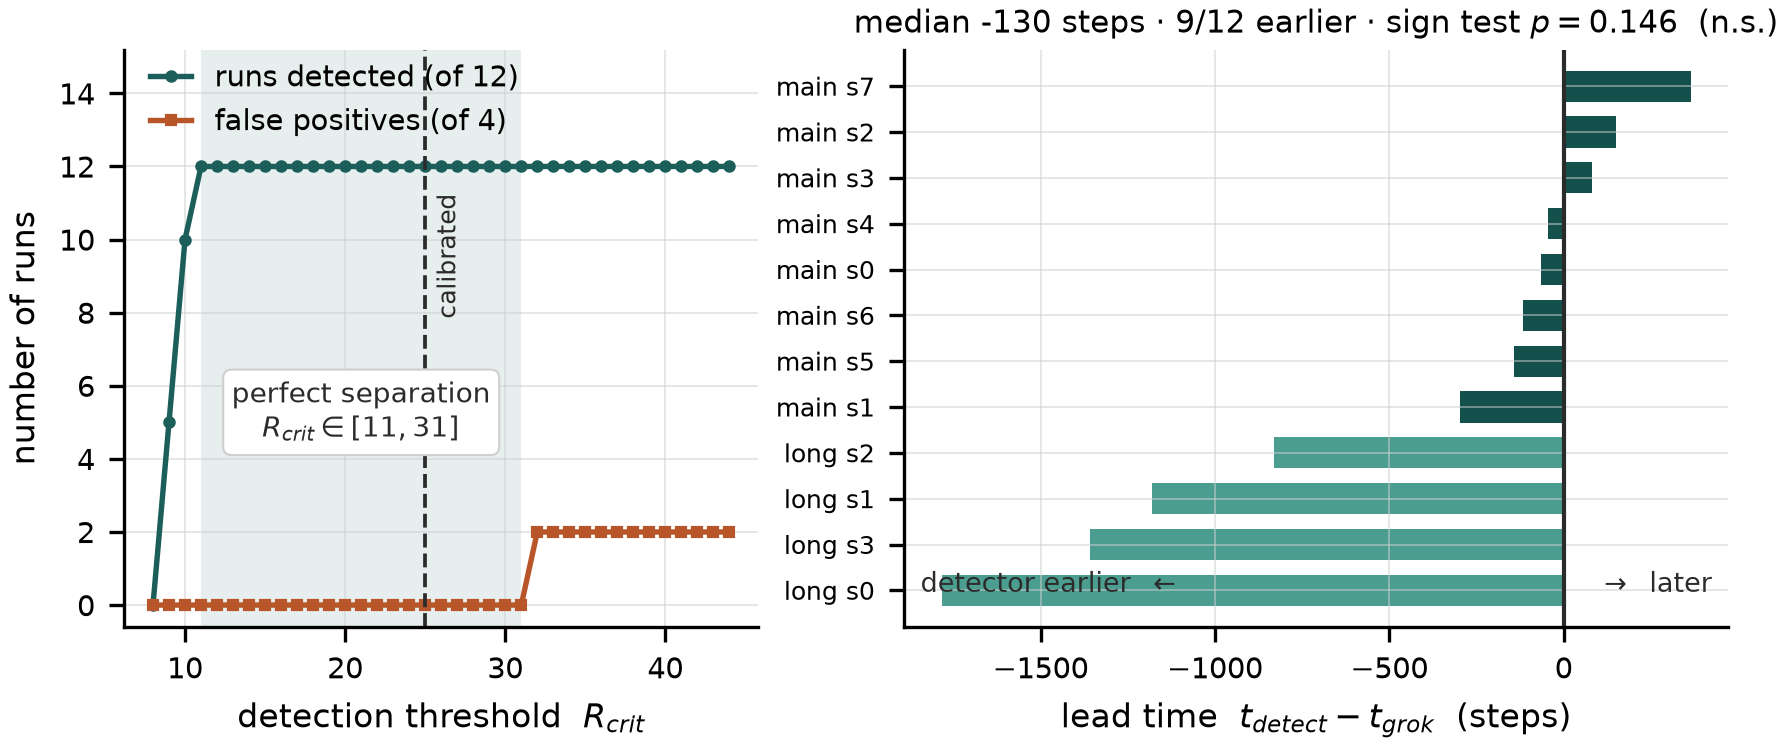
\includegraphics[width=\columnwidth]{../figures/fig3_detector.png}
	\caption{Left: detections and false positives against the threshold; the shaded band is
		the interval of perfect separation, $[11,31]$. Right: lead time per run. Median $-130$
		steps, $9/12$ negative, exact two-sided sign test $p=0.146$.}
\end{figure}

\begin{figure}[H]
	\centering
	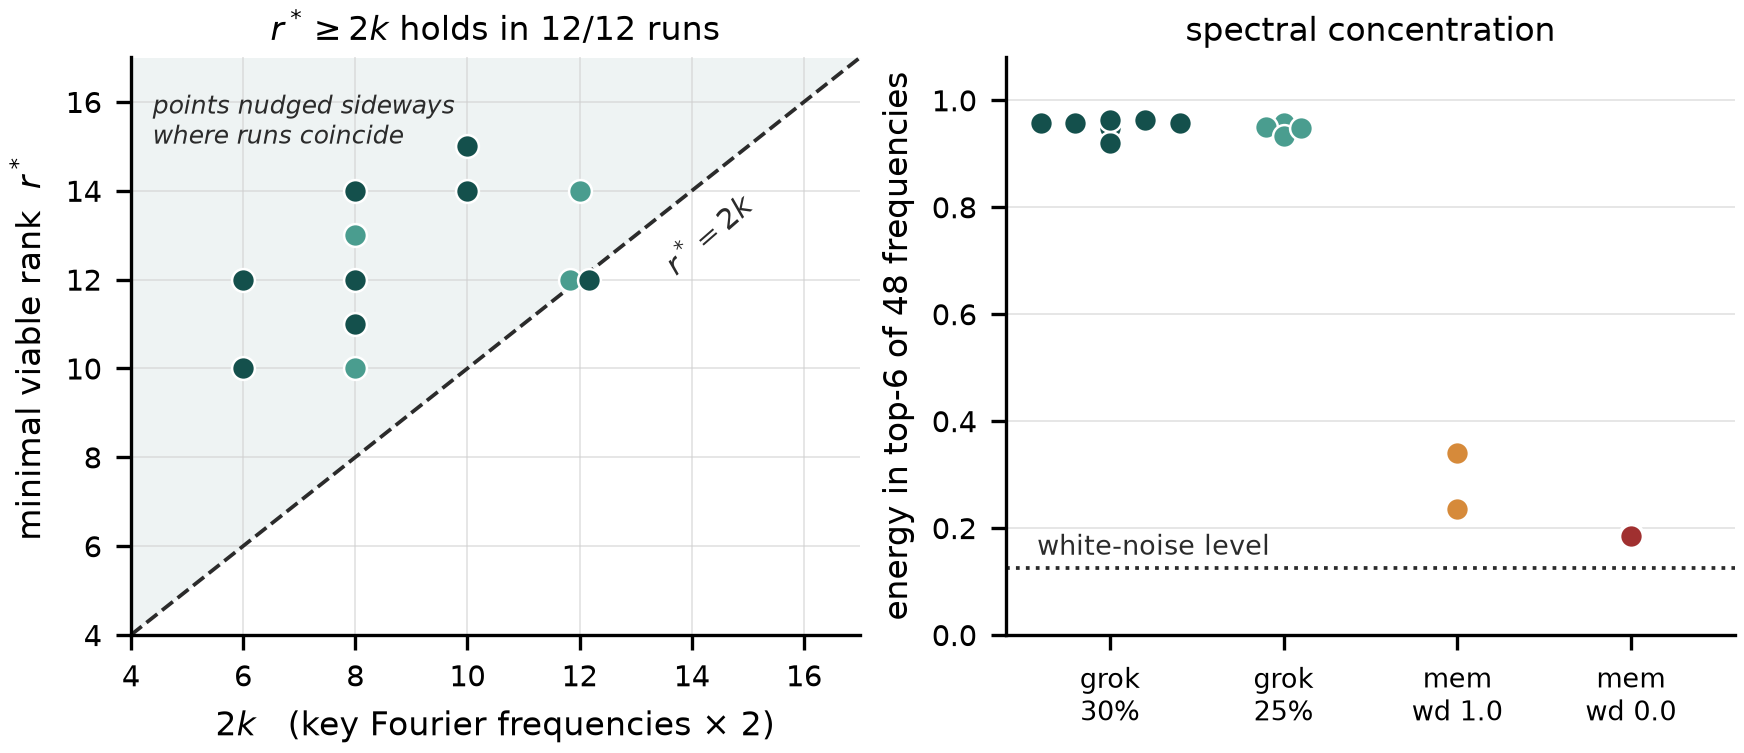
\includegraphics[width=\columnwidth]{../figures/fig4_fourier.png}
	\caption{Left: minimal viable rank against twice the number of key Fourier
		frequencies; all $12$ runs lie above $r^\star = 2k$ (points nudged sideways where runs
		coincide). Right: fraction of spectral energy in the top $6$ of $48$ frequencies.
		Pearson correlation between $2k$ and $r^\star$ is $+0.44$ ($p=0.152$, $n=12$): weak, as
		expected, since $2k$ is a lower bound and not a point prediction.}
	\label{fig:fourier}
\end{figure}


\begin{table}[h]
	\centering
	\caption{Sensitivity to the retention threshold. Trajectories were recomputed from
		scratch and $R_{\text{crit}}$ recalibrated with the same rule. Separation is complete
		in all three cases. The generalising group barely moves while the controls shift,
		indicating a sharp knee in the retention curve for generalising models only.}
	\label{tab:retention}
	\vskip 0.0in
	\begin{small}
		\begin{tabular}{lrrrrr}
			\toprule
			retention & $R_{\text{crit}}$ & gen. & \textsc{nc\_mem} & \textsc{nc\_wd0} & det./f.p. \\
			\midrule
			$0.80$ & $23$ & $10$--$14$ & $30$ & $72$--$75$ & $12/12$, $0/4$ \\
			$0.90$ & $25$ & $10$--$15$ & $33$--$34$ & $77$--$83$ & $12/12$, $0/4$ \\
			$0.95$ & $26$ & $10$--$15$ & $36$--$38$ & $80$--$86$ & $12/12$, $0/4$ \\
			\bottomrule
		\end{tabular}
	\end{small}
\end{table}

\begin{table}[H]
	\caption{Retained accuracy of the $12$ generalising anchors under rank truncation, on
		training and on held-out data (mean $\pm$ s.d.). The two accuracies track each other at every
		level, so truncation degrades the computed function rather than selectively removing
		generalisation. Test accuracy at rank $16$ equals its full-rank value.}
	\label{tab:ranktest}
	\vskip 0.15in
	\begin{center}
		\begin{small}
			\begin{tabular}{rcc}
				\toprule
				rank & train & test \\
				\midrule
				$8$   & $0.244 \pm .111$ & $0.244 \pm .105$ \\
				$10$  & $0.641 \pm .215$ & $0.635 \pm .214$ \\
				$12$  & $0.879 \pm .143$ & $0.871 \pm .146$ \\
				$14$  & $0.981 \pm .043$ & $0.977 \pm .049$ \\
				$16$  & $1.000 \pm .000$ & $0.9994 \pm .0008$ \\
				$128$ & $1.000 \pm .000$ & $0.9994 \pm .0008$ \\
				\bottomrule
			\end{tabular}
		\end{small}
	\end{center}
	\vskip -0.35in
\end{table}

\end{document}

